
% Default to the notebook output style

    


% Inherit from the specified cell style.




    
\documentclass[11pt]{article}

    
    
    \usepackage[T1]{fontenc}
    % Nicer default font (+ math font) than Computer Modern for most use cases
    \usepackage{mathpazo}

    % Basic figure setup, for now with no caption control since it's done
    % automatically by Pandoc (which extracts ![](path) syntax from Markdown).
    \usepackage{graphicx}
    % We will generate all images so they have a width \maxwidth. This means
    % that they will get their normal width if they fit onto the page, but
    % are scaled down if they would overflow the margins.
    \makeatletter
    \def\maxwidth{\ifdim\Gin@nat@width>\linewidth\linewidth
    \else\Gin@nat@width\fi}
    \makeatother
    \let\Oldincludegraphics\includegraphics
    % Set max figure width to be 80% of text width, for now hardcoded.
    \renewcommand{\includegraphics}[1]{\Oldincludegraphics[width=.8\maxwidth]{#1}}
    % Ensure that by default, figures have no caption (until we provide a
    % proper Figure object with a Caption API and a way to capture that
    % in the conversion process - todo).
    \usepackage{caption}
    \DeclareCaptionLabelFormat{nolabel}{}
    \captionsetup{labelformat=nolabel}

    \usepackage{adjustbox} % Used to constrain images to a maximum size 
    \usepackage{xcolor} % Allow colors to be defined
    \usepackage{enumerate} % Needed for markdown enumerations to work
    \usepackage{geometry} % Used to adjust the document margins
    \usepackage{amsmath} % Equations
    \usepackage{amssymb} % Equations
    \usepackage{textcomp} % defines textquotesingle
    % Hack from http://tex.stackexchange.com/a/47451/13684:
    \AtBeginDocument{%
        \def\PYZsq{\textquotesingle}% Upright quotes in Pygmentized code
    }
    \usepackage{upquote} % Upright quotes for verbatim code
    \usepackage{eurosym} % defines \euro
    \usepackage[mathletters]{ucs} % Extended unicode (utf-8) support
    \usepackage[utf8x]{inputenc} % Allow utf-8 characters in the tex document
    \usepackage{fancyvrb} % verbatim replacement that allows latex
    \usepackage{grffile} % extends the file name processing of package graphics 
                         % to support a larger range 
    % The hyperref package gives us a pdf with properly built
    % internal navigation ('pdf bookmarks' for the table of contents,
    % internal cross-reference links, web links for URLs, etc.)
    \usepackage{hyperref}
    \usepackage{longtable} % longtable support required by pandoc >1.10
    \usepackage{booktabs}  % table support for pandoc > 1.12.2
    \usepackage[inline]{enumitem} % IRkernel/repr support (it uses the enumerate* environment)
    \usepackage[normalem]{ulem} % ulem is needed to support strikethroughs (\sout)
                                % normalem makes italics be italics, not underlines
    

    
    
    % Colors for the hyperref package
    \definecolor{urlcolor}{rgb}{0,.145,.698}
    \definecolor{linkcolor}{rgb}{.71,0.21,0.01}
    \definecolor{citecolor}{rgb}{.12,.54,.11}

    % ANSI colors
    \definecolor{ansi-black}{HTML}{3E424D}
    \definecolor{ansi-black-intense}{HTML}{282C36}
    \definecolor{ansi-red}{HTML}{E75C58}
    \definecolor{ansi-red-intense}{HTML}{B22B31}
    \definecolor{ansi-green}{HTML}{00A250}
    \definecolor{ansi-green-intense}{HTML}{007427}
    \definecolor{ansi-yellow}{HTML}{DDB62B}
    \definecolor{ansi-yellow-intense}{HTML}{B27D12}
    \definecolor{ansi-blue}{HTML}{208FFB}
    \definecolor{ansi-blue-intense}{HTML}{0065CA}
    \definecolor{ansi-magenta}{HTML}{D160C4}
    \definecolor{ansi-magenta-intense}{HTML}{A03196}
    \definecolor{ansi-cyan}{HTML}{60C6C8}
    \definecolor{ansi-cyan-intense}{HTML}{258F8F}
    \definecolor{ansi-white}{HTML}{C5C1B4}
    \definecolor{ansi-white-intense}{HTML}{A1A6B2}

    % commands and environments needed by pandoc snippets
    % extracted from the output of `pandoc -s`
    \providecommand{\tightlist}{%
      \setlength{\itemsep}{0pt}\setlength{\parskip}{0pt}}
    \DefineVerbatimEnvironment{Highlighting}{Verbatim}{commandchars=\\\{\}}
    % Add ',fontsize=\small' for more characters per line
    \newenvironment{Shaded}{}{}
    \newcommand{\KeywordTok}[1]{\textcolor[rgb]{0.00,0.44,0.13}{\textbf{{#1}}}}
    \newcommand{\DataTypeTok}[1]{\textcolor[rgb]{0.56,0.13,0.00}{{#1}}}
    \newcommand{\DecValTok}[1]{\textcolor[rgb]{0.25,0.63,0.44}{{#1}}}
    \newcommand{\BaseNTok}[1]{\textcolor[rgb]{0.25,0.63,0.44}{{#1}}}
    \newcommand{\FloatTok}[1]{\textcolor[rgb]{0.25,0.63,0.44}{{#1}}}
    \newcommand{\CharTok}[1]{\textcolor[rgb]{0.25,0.44,0.63}{{#1}}}
    \newcommand{\StringTok}[1]{\textcolor[rgb]{0.25,0.44,0.63}{{#1}}}
    \newcommand{\CommentTok}[1]{\textcolor[rgb]{0.38,0.63,0.69}{\textit{{#1}}}}
    \newcommand{\OtherTok}[1]{\textcolor[rgb]{0.00,0.44,0.13}{{#1}}}
    \newcommand{\AlertTok}[1]{\textcolor[rgb]{1.00,0.00,0.00}{\textbf{{#1}}}}
    \newcommand{\FunctionTok}[1]{\textcolor[rgb]{0.02,0.16,0.49}{{#1}}}
    \newcommand{\RegionMarkerTok}[1]{{#1}}
    \newcommand{\ErrorTok}[1]{\textcolor[rgb]{1.00,0.00,0.00}{\textbf{{#1}}}}
    \newcommand{\NormalTok}[1]{{#1}}
    
    % Additional commands for more recent versions of Pandoc
    \newcommand{\ConstantTok}[1]{\textcolor[rgb]{0.53,0.00,0.00}{{#1}}}
    \newcommand{\SpecialCharTok}[1]{\textcolor[rgb]{0.25,0.44,0.63}{{#1}}}
    \newcommand{\VerbatimStringTok}[1]{\textcolor[rgb]{0.25,0.44,0.63}{{#1}}}
    \newcommand{\SpecialStringTok}[1]{\textcolor[rgb]{0.73,0.40,0.53}{{#1}}}
    \newcommand{\ImportTok}[1]{{#1}}
    \newcommand{\DocumentationTok}[1]{\textcolor[rgb]{0.73,0.13,0.13}{\textit{{#1}}}}
    \newcommand{\AnnotationTok}[1]{\textcolor[rgb]{0.38,0.63,0.69}{\textbf{\textit{{#1}}}}}
    \newcommand{\CommentVarTok}[1]{\textcolor[rgb]{0.38,0.63,0.69}{\textbf{\textit{{#1}}}}}
    \newcommand{\VariableTok}[1]{\textcolor[rgb]{0.10,0.09,0.49}{{#1}}}
    \newcommand{\ControlFlowTok}[1]{\textcolor[rgb]{0.00,0.44,0.13}{\textbf{{#1}}}}
    \newcommand{\OperatorTok}[1]{\textcolor[rgb]{0.40,0.40,0.40}{{#1}}}
    \newcommand{\BuiltInTok}[1]{{#1}}
    \newcommand{\ExtensionTok}[1]{{#1}}
    \newcommand{\PreprocessorTok}[1]{\textcolor[rgb]{0.74,0.48,0.00}{{#1}}}
    \newcommand{\AttributeTok}[1]{\textcolor[rgb]{0.49,0.56,0.16}{{#1}}}
    \newcommand{\InformationTok}[1]{\textcolor[rgb]{0.38,0.63,0.69}{\textbf{\textit{{#1}}}}}
    \newcommand{\WarningTok}[1]{\textcolor[rgb]{0.38,0.63,0.69}{\textbf{\textit{{#1}}}}}
    
    
    % Define a nice break command that doesn't care if a line doesn't already
    % exist.
    \def\br{\hspace*{\fill} \\* }
    % Math Jax compatability definitions
    \def\gt{>}
    \def\lt{<}
    % Document parameters
    \title{hw2.0\_tfidf\_classifier}
    
    
    

    % Pygments definitions
    
\makeatletter
\def\PY@reset{\let\PY@it=\relax \let\PY@bf=\relax%
    \let\PY@ul=\relax \let\PY@tc=\relax%
    \let\PY@bc=\relax \let\PY@ff=\relax}
\def\PY@tok#1{\csname PY@tok@#1\endcsname}
\def\PY@toks#1+{\ifx\relax#1\empty\else%
    \PY@tok{#1}\expandafter\PY@toks\fi}
\def\PY@do#1{\PY@bc{\PY@tc{\PY@ul{%
    \PY@it{\PY@bf{\PY@ff{#1}}}}}}}
\def\PY#1#2{\PY@reset\PY@toks#1+\relax+\PY@do{#2}}

\expandafter\def\csname PY@tok@w\endcsname{\def\PY@tc##1{\textcolor[rgb]{0.73,0.73,0.73}{##1}}}
\expandafter\def\csname PY@tok@c\endcsname{\let\PY@it=\textit\def\PY@tc##1{\textcolor[rgb]{0.25,0.50,0.50}{##1}}}
\expandafter\def\csname PY@tok@cp\endcsname{\def\PY@tc##1{\textcolor[rgb]{0.74,0.48,0.00}{##1}}}
\expandafter\def\csname PY@tok@k\endcsname{\let\PY@bf=\textbf\def\PY@tc##1{\textcolor[rgb]{0.00,0.50,0.00}{##1}}}
\expandafter\def\csname PY@tok@kp\endcsname{\def\PY@tc##1{\textcolor[rgb]{0.00,0.50,0.00}{##1}}}
\expandafter\def\csname PY@tok@kt\endcsname{\def\PY@tc##1{\textcolor[rgb]{0.69,0.00,0.25}{##1}}}
\expandafter\def\csname PY@tok@o\endcsname{\def\PY@tc##1{\textcolor[rgb]{0.40,0.40,0.40}{##1}}}
\expandafter\def\csname PY@tok@ow\endcsname{\let\PY@bf=\textbf\def\PY@tc##1{\textcolor[rgb]{0.67,0.13,1.00}{##1}}}
\expandafter\def\csname PY@tok@nb\endcsname{\def\PY@tc##1{\textcolor[rgb]{0.00,0.50,0.00}{##1}}}
\expandafter\def\csname PY@tok@nf\endcsname{\def\PY@tc##1{\textcolor[rgb]{0.00,0.00,1.00}{##1}}}
\expandafter\def\csname PY@tok@nc\endcsname{\let\PY@bf=\textbf\def\PY@tc##1{\textcolor[rgb]{0.00,0.00,1.00}{##1}}}
\expandafter\def\csname PY@tok@nn\endcsname{\let\PY@bf=\textbf\def\PY@tc##1{\textcolor[rgb]{0.00,0.00,1.00}{##1}}}
\expandafter\def\csname PY@tok@ne\endcsname{\let\PY@bf=\textbf\def\PY@tc##1{\textcolor[rgb]{0.82,0.25,0.23}{##1}}}
\expandafter\def\csname PY@tok@nv\endcsname{\def\PY@tc##1{\textcolor[rgb]{0.10,0.09,0.49}{##1}}}
\expandafter\def\csname PY@tok@no\endcsname{\def\PY@tc##1{\textcolor[rgb]{0.53,0.00,0.00}{##1}}}
\expandafter\def\csname PY@tok@nl\endcsname{\def\PY@tc##1{\textcolor[rgb]{0.63,0.63,0.00}{##1}}}
\expandafter\def\csname PY@tok@ni\endcsname{\let\PY@bf=\textbf\def\PY@tc##1{\textcolor[rgb]{0.60,0.60,0.60}{##1}}}
\expandafter\def\csname PY@tok@na\endcsname{\def\PY@tc##1{\textcolor[rgb]{0.49,0.56,0.16}{##1}}}
\expandafter\def\csname PY@tok@nt\endcsname{\let\PY@bf=\textbf\def\PY@tc##1{\textcolor[rgb]{0.00,0.50,0.00}{##1}}}
\expandafter\def\csname PY@tok@nd\endcsname{\def\PY@tc##1{\textcolor[rgb]{0.67,0.13,1.00}{##1}}}
\expandafter\def\csname PY@tok@s\endcsname{\def\PY@tc##1{\textcolor[rgb]{0.73,0.13,0.13}{##1}}}
\expandafter\def\csname PY@tok@sd\endcsname{\let\PY@it=\textit\def\PY@tc##1{\textcolor[rgb]{0.73,0.13,0.13}{##1}}}
\expandafter\def\csname PY@tok@si\endcsname{\let\PY@bf=\textbf\def\PY@tc##1{\textcolor[rgb]{0.73,0.40,0.53}{##1}}}
\expandafter\def\csname PY@tok@se\endcsname{\let\PY@bf=\textbf\def\PY@tc##1{\textcolor[rgb]{0.73,0.40,0.13}{##1}}}
\expandafter\def\csname PY@tok@sr\endcsname{\def\PY@tc##1{\textcolor[rgb]{0.73,0.40,0.53}{##1}}}
\expandafter\def\csname PY@tok@ss\endcsname{\def\PY@tc##1{\textcolor[rgb]{0.10,0.09,0.49}{##1}}}
\expandafter\def\csname PY@tok@sx\endcsname{\def\PY@tc##1{\textcolor[rgb]{0.00,0.50,0.00}{##1}}}
\expandafter\def\csname PY@tok@m\endcsname{\def\PY@tc##1{\textcolor[rgb]{0.40,0.40,0.40}{##1}}}
\expandafter\def\csname PY@tok@gh\endcsname{\let\PY@bf=\textbf\def\PY@tc##1{\textcolor[rgb]{0.00,0.00,0.50}{##1}}}
\expandafter\def\csname PY@tok@gu\endcsname{\let\PY@bf=\textbf\def\PY@tc##1{\textcolor[rgb]{0.50,0.00,0.50}{##1}}}
\expandafter\def\csname PY@tok@gd\endcsname{\def\PY@tc##1{\textcolor[rgb]{0.63,0.00,0.00}{##1}}}
\expandafter\def\csname PY@tok@gi\endcsname{\def\PY@tc##1{\textcolor[rgb]{0.00,0.63,0.00}{##1}}}
\expandafter\def\csname PY@tok@gr\endcsname{\def\PY@tc##1{\textcolor[rgb]{1.00,0.00,0.00}{##1}}}
\expandafter\def\csname PY@tok@ge\endcsname{\let\PY@it=\textit}
\expandafter\def\csname PY@tok@gs\endcsname{\let\PY@bf=\textbf}
\expandafter\def\csname PY@tok@gp\endcsname{\let\PY@bf=\textbf\def\PY@tc##1{\textcolor[rgb]{0.00,0.00,0.50}{##1}}}
\expandafter\def\csname PY@tok@go\endcsname{\def\PY@tc##1{\textcolor[rgb]{0.53,0.53,0.53}{##1}}}
\expandafter\def\csname PY@tok@gt\endcsname{\def\PY@tc##1{\textcolor[rgb]{0.00,0.27,0.87}{##1}}}
\expandafter\def\csname PY@tok@err\endcsname{\def\PY@bc##1{\setlength{\fboxsep}{0pt}\fcolorbox[rgb]{1.00,0.00,0.00}{1,1,1}{\strut ##1}}}
\expandafter\def\csname PY@tok@kc\endcsname{\let\PY@bf=\textbf\def\PY@tc##1{\textcolor[rgb]{0.00,0.50,0.00}{##1}}}
\expandafter\def\csname PY@tok@kd\endcsname{\let\PY@bf=\textbf\def\PY@tc##1{\textcolor[rgb]{0.00,0.50,0.00}{##1}}}
\expandafter\def\csname PY@tok@kn\endcsname{\let\PY@bf=\textbf\def\PY@tc##1{\textcolor[rgb]{0.00,0.50,0.00}{##1}}}
\expandafter\def\csname PY@tok@kr\endcsname{\let\PY@bf=\textbf\def\PY@tc##1{\textcolor[rgb]{0.00,0.50,0.00}{##1}}}
\expandafter\def\csname PY@tok@bp\endcsname{\def\PY@tc##1{\textcolor[rgb]{0.00,0.50,0.00}{##1}}}
\expandafter\def\csname PY@tok@fm\endcsname{\def\PY@tc##1{\textcolor[rgb]{0.00,0.00,1.00}{##1}}}
\expandafter\def\csname PY@tok@vc\endcsname{\def\PY@tc##1{\textcolor[rgb]{0.10,0.09,0.49}{##1}}}
\expandafter\def\csname PY@tok@vg\endcsname{\def\PY@tc##1{\textcolor[rgb]{0.10,0.09,0.49}{##1}}}
\expandafter\def\csname PY@tok@vi\endcsname{\def\PY@tc##1{\textcolor[rgb]{0.10,0.09,0.49}{##1}}}
\expandafter\def\csname PY@tok@vm\endcsname{\def\PY@tc##1{\textcolor[rgb]{0.10,0.09,0.49}{##1}}}
\expandafter\def\csname PY@tok@sa\endcsname{\def\PY@tc##1{\textcolor[rgb]{0.73,0.13,0.13}{##1}}}
\expandafter\def\csname PY@tok@sb\endcsname{\def\PY@tc##1{\textcolor[rgb]{0.73,0.13,0.13}{##1}}}
\expandafter\def\csname PY@tok@sc\endcsname{\def\PY@tc##1{\textcolor[rgb]{0.73,0.13,0.13}{##1}}}
\expandafter\def\csname PY@tok@dl\endcsname{\def\PY@tc##1{\textcolor[rgb]{0.73,0.13,0.13}{##1}}}
\expandafter\def\csname PY@tok@s2\endcsname{\def\PY@tc##1{\textcolor[rgb]{0.73,0.13,0.13}{##1}}}
\expandafter\def\csname PY@tok@sh\endcsname{\def\PY@tc##1{\textcolor[rgb]{0.73,0.13,0.13}{##1}}}
\expandafter\def\csname PY@tok@s1\endcsname{\def\PY@tc##1{\textcolor[rgb]{0.73,0.13,0.13}{##1}}}
\expandafter\def\csname PY@tok@mb\endcsname{\def\PY@tc##1{\textcolor[rgb]{0.40,0.40,0.40}{##1}}}
\expandafter\def\csname PY@tok@mf\endcsname{\def\PY@tc##1{\textcolor[rgb]{0.40,0.40,0.40}{##1}}}
\expandafter\def\csname PY@tok@mh\endcsname{\def\PY@tc##1{\textcolor[rgb]{0.40,0.40,0.40}{##1}}}
\expandafter\def\csname PY@tok@mi\endcsname{\def\PY@tc##1{\textcolor[rgb]{0.40,0.40,0.40}{##1}}}
\expandafter\def\csname PY@tok@il\endcsname{\def\PY@tc##1{\textcolor[rgb]{0.40,0.40,0.40}{##1}}}
\expandafter\def\csname PY@tok@mo\endcsname{\def\PY@tc##1{\textcolor[rgb]{0.40,0.40,0.40}{##1}}}
\expandafter\def\csname PY@tok@ch\endcsname{\let\PY@it=\textit\def\PY@tc##1{\textcolor[rgb]{0.25,0.50,0.50}{##1}}}
\expandafter\def\csname PY@tok@cm\endcsname{\let\PY@it=\textit\def\PY@tc##1{\textcolor[rgb]{0.25,0.50,0.50}{##1}}}
\expandafter\def\csname PY@tok@cpf\endcsname{\let\PY@it=\textit\def\PY@tc##1{\textcolor[rgb]{0.25,0.50,0.50}{##1}}}
\expandafter\def\csname PY@tok@c1\endcsname{\let\PY@it=\textit\def\PY@tc##1{\textcolor[rgb]{0.25,0.50,0.50}{##1}}}
\expandafter\def\csname PY@tok@cs\endcsname{\let\PY@it=\textit\def\PY@tc##1{\textcolor[rgb]{0.25,0.50,0.50}{##1}}}

\def\PYZbs{\char`\\}
\def\PYZus{\char`\_}
\def\PYZob{\char`\{}
\def\PYZcb{\char`\}}
\def\PYZca{\char`\^}
\def\PYZam{\char`\&}
\def\PYZlt{\char`\<}
\def\PYZgt{\char`\>}
\def\PYZsh{\char`\#}
\def\PYZpc{\char`\%}
\def\PYZdl{\char`\$}
\def\PYZhy{\char`\-}
\def\PYZsq{\char`\'}
\def\PYZdq{\char`\"}
\def\PYZti{\char`\~}
% for compatibility with earlier versions
\def\PYZat{@}
\def\PYZlb{[}
\def\PYZrb{]}
\makeatother


    % Exact colors from NB
    \definecolor{incolor}{rgb}{0.0, 0.0, 0.5}
    \definecolor{outcolor}{rgb}{0.545, 0.0, 0.0}



    
    % Prevent overflowing lines due to hard-to-break entities
    \sloppy 
    % Setup hyperref package
    \hypersetup{
      breaklinks=true,  % so long urls are correctly broken across lines
      colorlinks=true,
      urlcolor=urlcolor,
      linkcolor=linkcolor,
      citecolor=citecolor,
      }
    % Slightly bigger margins than the latex defaults
    
    \geometry{verbose,tmargin=1in,bmargin=1in,lmargin=1in,rmargin=1in}
    
    

    \begin{document}
    
    
    \maketitle
    
    

    
    \section{Homework 2 - TF-IDF
Classifier}\label{homework-2---tf-idf-classifier}

Ваша цель обучить классификатор который будет находить "токсичные"
комментарии и опубликовать решения на Kaggle
\href{https://www.kaggle.com/c/jigsaw-toxic-comment-classification-challenge}{Toxic
Comment Classification Challenge}

В процессе обучения нужно ответить на
\textbf{\emph{\href{https://docs.google.com/forms/d/e/1FAIpQLSd9mQx8EFpSH6FhCy1M_FmISzy3lhgyyqV3TN0pmtop7slmTA/viewform?usp=sf_link}{вопросы}}}

Данные можно скачать тут -
https://www.kaggle.com/c/jigsaw-toxic-comment-classification-challenge/data

    \begin{Verbatim}[commandchars=\\\{\}]
{\color{incolor}In [{\color{incolor}1}]:} \PY{k+kn}{import} \PY{n+nn}{numpy} \PY{k}{as} \PY{n+nn}{np}
        \PY{k+kn}{import} \PY{n+nn}{pandas} \PY{k}{as} \PY{n+nn}{pd}
        \PY{k+kn}{import} \PY{n+nn}{re}
        
        \PY{k+kn}{from} \PY{n+nn}{string} \PY{k}{import} \PY{n}{punctuation}
        \PY{k+kn}{from} \PY{n+nn}{wordcloud} \PY{k}{import} \PY{n}{STOPWORDS}
        \PY{k+kn}{from} \PY{n+nn}{collections} \PY{k}{import} \PY{n}{Counter}
        
        \PY{k+kn}{from} \PY{n+nn}{scipy}\PY{n+nn}{.}\PY{n+nn}{sparse} \PY{k}{import} \PY{n}{csr\PYZus{}matrix}\PY{p}{,} \PY{n}{hstack}
        \PY{k+kn}{from} \PY{n+nn}{sklearn}\PY{n+nn}{.}\PY{n+nn}{feature\PYZus{}extraction}\PY{n+nn}{.}\PY{n+nn}{text} \PY{k}{import} \PY{n}{TfidfVectorizer}\PY{p}{,} \PY{n}{CountVectorizer}
        \PY{k+kn}{from} \PY{n+nn}{sklearn}\PY{n+nn}{.}\PY{n+nn}{linear\PYZus{}model} \PY{k}{import} \PY{n}{LogisticRegression}
        \PY{k+kn}{from} \PY{n+nn}{sklearn}\PY{n+nn}{.}\PY{n+nn}{model\PYZus{}selection} \PY{k}{import} \PY{n}{cross\PYZus{}val\PYZus{}score}
\end{Verbatim}


    \begin{Verbatim}[commandchars=\\\{\}]
{\color{incolor}In [{\color{incolor}2}]:} \PY{n}{class\PYZus{}names} \PY{o}{=} \PY{p}{[}\PY{l+s+s1}{\PYZsq{}}\PY{l+s+s1}{toxic}\PY{l+s+s1}{\PYZsq{}}\PY{p}{,} \PY{l+s+s1}{\PYZsq{}}\PY{l+s+s1}{severe\PYZus{}toxic}\PY{l+s+s1}{\PYZsq{}}\PY{p}{,} \PY{l+s+s1}{\PYZsq{}}\PY{l+s+s1}{obscene}\PY{l+s+s1}{\PYZsq{}}\PY{p}{,} \PY{l+s+s1}{\PYZsq{}}\PY{l+s+s1}{threat}\PY{l+s+s1}{\PYZsq{}}\PY{p}{,} \PY{l+s+s1}{\PYZsq{}}\PY{l+s+s1}{insult}\PY{l+s+s1}{\PYZsq{}}\PY{p}{,} \PY{l+s+s1}{\PYZsq{}}\PY{l+s+s1}{identity\PYZus{}hate}\PY{l+s+s1}{\PYZsq{}}\PY{p}{]}
        
        \PY{n}{train} \PY{o}{=} \PY{n}{pd}\PY{o}{.}\PY{n}{read\PYZus{}csv}\PY{p}{(}\PY{l+s+s1}{\PYZsq{}}\PY{l+s+s1}{../../data/Toxis comments/train.csv}\PY{l+s+s1}{\PYZsq{}}\PY{p}{)}\PY{o}{.}\PY{n}{fillna}\PY{p}{(}\PY{l+s+s1}{\PYZsq{}}\PY{l+s+s1}{ }\PY{l+s+s1}{\PYZsq{}}\PY{p}{)}
        \PY{n}{test} \PY{o}{=} \PY{n}{pd}\PY{o}{.}\PY{n}{read\PYZus{}csv}\PY{p}{(}\PY{l+s+s1}{\PYZsq{}}\PY{l+s+s1}{../../data/Toxis comments/test.csv}\PY{l+s+s1}{\PYZsq{}}\PY{p}{)}\PY{o}{.}\PY{n}{fillna}\PY{p}{(}\PY{l+s+s1}{\PYZsq{}}\PY{l+s+s1}{ }\PY{l+s+s1}{\PYZsq{}}\PY{p}{)}
\end{Verbatim}


    \begin{Verbatim}[commandchars=\\\{\}]
{\color{incolor}In [{\color{incolor}3}]:} \PY{n}{train}\PY{o}{.}\PY{n}{shape}
\end{Verbatim}


\begin{Verbatim}[commandchars=\\\{\}]
{\color{outcolor}Out[{\color{outcolor}3}]:} (159571, 8)
\end{Verbatim}
            
    Стадартными подходами для анализа текста являются
\href{https://en.wikipedia.org/wiki/Bag-of-words_model}{Bag of words} и
его модификация
\href{https://en.wikipedia.org/wiki/Tf\%E2\%80\%93idf}{TF-IDF}.

Они реалзованны в \texttt{sklearn} в виде
\href{http://scikit-learn.org/stable/modules/generated/sklearn.feature_extraction.text.CountVectorizer.html}{CountVectorizer}
и
\href{http://scikit-learn.org/stable/modules/generated/sklearn.feature_extraction.text.TfidfVectorizer.html}{TfidfVectorizer}.

Более подробней про них можно посмотреть
\href{https://github.com/udsclub/workshop/blob/master/notebooks/UDS-workshop-feature-extraction-and-engineering.ipynb}{тут}

    \begin{Verbatim}[commandchars=\\\{\}]
{\color{incolor}In [{\color{incolor}4}]:} \PY{n}{train\PYZus{}text} \PY{o}{=} \PY{n}{train}\PY{p}{[}\PY{l+s+s1}{\PYZsq{}}\PY{l+s+s1}{comment\PYZus{}text}\PY{l+s+s1}{\PYZsq{}}\PY{p}{]}
        \PY{n}{test\PYZus{}text} \PY{o}{=} \PY{n}{test}\PY{p}{[}\PY{l+s+s1}{\PYZsq{}}\PY{l+s+s1}{comment\PYZus{}text}\PY{l+s+s1}{\PYZsq{}}\PY{p}{]}
        \PY{n}{all\PYZus{}text} \PY{o}{=} \PY{n}{pd}\PY{o}{.}\PY{n}{concat}\PY{p}{(}\PY{p}{[}\PY{n}{train\PYZus{}text}\PY{p}{,} \PY{n}{test\PYZus{}text}\PY{p}{]}\PY{p}{)}
\end{Verbatim}


    \begin{Verbatim}[commandchars=\\\{\}]
{\color{incolor}In [{\color{incolor}5}]:} \PY{c+c1}{\PYZsh{} to count the most common words in the comments you should set max\PYZus{}features=1000 to avoid MemoryError}
        \PY{n}{word\PYZus{}vectorizer} \PY{o}{=} \PY{n}{TfidfVectorizer}\PY{p}{(}\PY{n}{analyzer}\PY{o}{=}\PY{l+s+s1}{\PYZsq{}}\PY{l+s+s1}{word}\PY{l+s+s1}{\PYZsq{}}\PY{p}{,}
                                          \PY{n}{max\PYZus{}features}\PY{o}{=}\PY{l+m+mi}{1000}\PY{p}{,}
                                         \PY{p}{)}
\end{Verbatim}


    \begin{Verbatim}[commandchars=\\\{\}]
{\color{incolor}In [{\color{incolor}6}]:} \PY{n}{all\PYZus{}word\PYZus{}features} \PY{o}{=} \PY{n}{word\PYZus{}vectorizer}\PY{o}{.}\PY{n}{fit\PYZus{}transform}\PY{p}{(}\PY{n}{all\PYZus{}text}\PY{p}{)}
        \PY{n}{x\PYZus{}train} \PY{o}{=} \PY{n}{word\PYZus{}vectorizer}\PY{o}{.}\PY{n}{transform}\PY{p}{(}\PY{n}{train\PYZus{}text}\PY{p}{)}
        \PY{n}{x\PYZus{}test} \PY{o}{=} \PY{n}{word\PYZus{}vectorizer}\PY{o}{.}\PY{n}{transform}\PY{p}{(}\PY{n}{test\PYZus{}text}\PY{p}{)}
\end{Verbatim}


    \section{What words are the most common in the
dataset}\label{what-words-are-the-most-common-in-the-dataset}

answer depends on what Vectorizer we have chosen. But the most common is
the same: 'the' \#\#\# First method:

    \begin{Verbatim}[commandchars=\\\{\}]
{\color{incolor}In [{\color{incolor}7}]:} \PY{n}{sums} \PY{o}{=} \PY{n}{all\PYZus{}word\PYZus{}features}\PY{o}{.}\PY{n}{todense}\PY{p}{(}\PY{p}{)}\PY{o}{.}\PY{n}{sum}\PY{p}{(}\PY{n}{axis}\PY{o}{=}\PY{l+m+mi}{0}\PY{p}{)}
        \PY{n}{d} \PY{o}{=} \PY{n+nb}{list}\PY{p}{(}\PY{n+nb}{zip}\PY{p}{(}\PY{n}{word\PYZus{}vectorizer}\PY{o}{.}\PY{n}{get\PYZus{}feature\PYZus{}names}\PY{p}{(}\PY{p}{)}\PY{p}{,} \PY{n}{sums}\PY{o}{.}\PY{n}{tolist}\PY{p}{(}\PY{p}{)}\PY{p}{[}\PY{l+m+mi}{0}\PY{p}{]}\PY{p}{)}\PY{p}{)}
        \PY{n}{words\PYZus{}sorted} \PY{o}{=} \PY{n+nb}{sorted}\PY{p}{(}\PY{n}{d}\PY{p}{,} \PY{n}{key}\PY{o}{=}\PY{k}{lambda} \PY{n}{x}\PY{p}{:} \PY{n}{x}\PY{p}{[}\PY{l+m+mi}{1}\PY{p}{]}\PY{p}{,} \PY{n}{reverse}\PY{o}{=}\PY{k+kc}{True}\PY{p}{)}
\end{Verbatim}


    \begin{Verbatim}[commandchars=\\\{\}]
{\color{incolor}In [{\color{incolor}8}]:} \PY{n}{words\PYZus{}sorted}\PY{p}{[}\PY{p}{:}\PY{l+m+mi}{5}\PY{p}{]}
\end{Verbatim}


\begin{Verbatim}[commandchars=\\\{\}]
{\color{outcolor}Out[{\color{outcolor}8}]:} [('the', 35525.038806166674),
         ('to', 23633.798627869706),
         ('you', 22468.364330022436),
         ('of', 19213.909587014077),
         ('and', 18905.674429729585)]
\end{Verbatim}
            
    \subsubsection{Second method:}\label{second-method}

    \begin{Verbatim}[commandchars=\\\{\}]
{\color{incolor}In [{\color{incolor}9}]:} \PY{k}{def} \PY{n+nf}{get\PYZus{}words}\PY{p}{(}\PY{n}{text}\PY{p}{)}\PY{p}{:}
            \PY{l+s+sd}{\PYZdq{}\PYZdq{}\PYZdq{}return list of the words\PYZdq{}\PYZdq{}\PYZdq{}}
            \PY{n}{pattern} \PY{o}{=} \PY{l+s+sa}{r}\PY{l+s+s1}{\PYZsq{}}\PY{l+s+s1}{[a\PYZhy{}z]+}\PY{l+s+s1}{\PYZsq{}}
            \PY{n}{words} \PY{o}{=} \PY{n}{re}\PY{o}{.}\PY{n}{findall}\PY{p}{(}\PY{n}{pattern}\PY{p}{,} \PY{n}{text}\PY{o}{.}\PY{n}{lower}\PY{p}{(}\PY{p}{)}\PY{p}{)}
            
            \PY{k}{return} \PY{n}{words}
\end{Verbatim}


    \begin{Verbatim}[commandchars=\\\{\}]
{\color{incolor}In [{\color{incolor}10}]:} \PY{n}{words\PYZus{}lists} \PY{o}{=} \PY{n}{all\PYZus{}text}\PY{o}{.}\PY{n}{apply}\PY{p}{(}\PY{n}{get\PYZus{}words}\PY{p}{)}
\end{Verbatim}


    \begin{Verbatim}[commandchars=\\\{\}]
{\color{incolor}In [{\color{incolor}11}]:} \PY{n}{all\PYZus{}words} \PY{o}{=} \PY{n+nb}{dict}\PY{p}{(}\PY{p}{)}
         
         \PY{k}{for} \PY{n}{item} \PY{o+ow}{in} \PY{n}{words\PYZus{}lists}\PY{p}{:}
             
             \PY{k}{for} \PY{n}{word} \PY{o+ow}{in} \PY{n+nb}{list}\PY{p}{(}\PY{n}{item}\PY{p}{)}\PY{p}{:}
                 \PY{k}{if} \PY{n}{word} \PY{o+ow}{in} \PY{n}{all\PYZus{}words}\PY{p}{:}
                     \PY{n}{all\PYZus{}words}\PY{p}{[}\PY{n}{word}\PY{p}{]} \PY{o}{+}\PY{o}{=} \PY{l+m+mi}{1}
                 \PY{k}{else}\PY{p}{:}
                     \PY{n}{all\PYZus{}words}\PY{p}{[}\PY{n}{word}\PY{p}{]} \PY{o}{=} \PY{l+m+mi}{1}
\end{Verbatim}


    \begin{Verbatim}[commandchars=\\\{\}]
{\color{incolor}In [{\color{incolor}12}]:} \PY{n+nb}{sorted}\PY{p}{(}\PY{n}{all\PYZus{}words}\PY{o}{.}\PY{n}{items}\PY{p}{(}\PY{p}{)}\PY{p}{,} \PY{n}{key}\PY{o}{=}\PY{k}{lambda} \PY{n}{x}\PY{p}{:} \PY{n}{x}\PY{p}{[}\PY{l+m+mi}{1}\PY{p}{]}\PY{p}{,} \PY{n}{reverse}\PY{o}{=}\PY{k+kc}{True}\PY{p}{)}\PY{p}{[}\PY{p}{:}\PY{l+m+mi}{5}\PY{p}{]}
\end{Verbatim}


\begin{Verbatim}[commandchars=\\\{\}]
{\color{outcolor}Out[{\color{outcolor}12}]:} [('the', 919075), ('to', 539244), ('i', 434390), ('a', 412567), ('of', 410841)]
\end{Verbatim}
            
    \subsection{Third}\label{third}

    \begin{Verbatim}[commandchars=\\\{\}]
{\color{incolor}In [{\color{incolor}13}]:} \PY{n}{result} \PY{o}{=} \PY{n}{Counter}\PY{p}{(}\PY{n}{all\PYZus{}words}\PY{p}{)}
         \PY{n}{result}\PY{o}{.}\PY{n}{most\PYZus{}common}\PY{p}{(}\PY{l+m+mi}{5}\PY{p}{)}
\end{Verbatim}


\begin{Verbatim}[commandchars=\\\{\}]
{\color{outcolor}Out[{\color{outcolor}13}]:} [('the', 919075), ('to', 539244), ('i', 434390), ('a', 412567), ('of', 410841)]
\end{Verbatim}
            
    \section{Logistic regression}\label{logistic-regression}

    Для классификации будем использовать логистическую регрессию
\href{http://scikit-learn.org/stable/modules/generated/sklearn.linear_model.LogisticRegression.html}{LogisticRegression}.

    Будем тренировать по одному классификатору на каждый класс.

Что бы провалидировать качество модели воспользуемся функцией
\href{http://scikit-learn.org/stable/modules/generated/sklearn.model_selection.cross_val_score.html}{cross\_val\_score}

    \subsubsection{add some features to train and test
datasets}\label{add-some-features-to-train-and-test-datasets}

*don't make our predictions better

    \begin{Verbatim}[commandchars=\\\{\}]
{\color{incolor}In [{\color{incolor}14}]:} \PY{n}{add\PYZus{}more\PYZus{}features} \PY{o}{=} \PY{k+kc}{False}
\end{Verbatim}


    \begin{Verbatim}[commandchars=\\\{\}]
{\color{incolor}In [{\color{incolor}15}]:} \PY{k}{if} \PY{n}{add\PYZus{}more\PYZus{}features}\PY{p}{:}
             \PY{c+c1}{\PYZsh{} TRAIN}
         
             \PY{n}{train}\PY{p}{[}\PY{l+s+s1}{\PYZsq{}}\PY{l+s+s1}{count\PYZus{}word}\PY{l+s+s1}{\PYZsq{}}\PY{p}{]}\PY{o}{=}\PY{n}{train}\PY{p}{[}\PY{l+s+s2}{\PYZdq{}}\PY{l+s+s2}{comment\PYZus{}text}\PY{l+s+s2}{\PYZdq{}}\PY{p}{]}\PY{o}{.}\PY{n}{apply}\PY{p}{(}\PY{k}{lambda} \PY{n}{x}\PY{p}{:} \PY{n+nb}{len}\PY{p}{(}\PY{n+nb}{str}\PY{p}{(}\PY{n}{x}\PY{p}{)}\PY{o}{.}\PY{n}{split}\PY{p}{(}\PY{p}{)}\PY{p}{)}\PY{p}{)}
             \PY{c+c1}{\PYZsh{}Unique word count}
             \PY{n}{train}\PY{p}{[}\PY{l+s+s1}{\PYZsq{}}\PY{l+s+s1}{count\PYZus{}unique\PYZus{}word}\PY{l+s+s1}{\PYZsq{}}\PY{p}{]}\PY{o}{=}\PY{n}{train}\PY{p}{[}\PY{l+s+s2}{\PYZdq{}}\PY{l+s+s2}{comment\PYZus{}text}\PY{l+s+s2}{\PYZdq{}}\PY{p}{]}\PY{o}{.}\PY{n}{apply}\PY{p}{(}\PY{k}{lambda} \PY{n}{x}\PY{p}{:} \PY{n+nb}{len}\PY{p}{(}\PY{n+nb}{set}\PY{p}{(}\PY{n+nb}{str}\PY{p}{(}\PY{n}{x}\PY{p}{)}\PY{o}{.}\PY{n}{split}\PY{p}{(}\PY{p}{)}\PY{p}{)}\PY{p}{)}\PY{p}{)}
             \PY{c+c1}{\PYZsh{}punctuation count}
             \PY{n}{train}\PY{p}{[}\PY{l+s+s2}{\PYZdq{}}\PY{l+s+s2}{count\PYZus{}punctuations}\PY{l+s+s2}{\PYZdq{}}\PY{p}{]} \PY{o}{=}\PY{n}{train}\PY{p}{[}\PY{l+s+s2}{\PYZdq{}}\PY{l+s+s2}{comment\PYZus{}text}\PY{l+s+s2}{\PYZdq{}}\PY{p}{]}\PY{o}{.}\PY{n}{apply}\PY{p}{(}\PY{k}{lambda} \PY{n}{x}\PY{p}{:} \PY{n+nb}{len}\PY{p}{(}\PY{p}{[}\PY{n}{c} \PY{k}{for} \PY{n}{c} \PY{o+ow}{in} \PY{n+nb}{str}\PY{p}{(}\PY{n}{x}\PY{p}{)} \PY{k}{if} \PY{n}{c} \PY{o+ow}{in} \PY{n}{punctuation}\PY{p}{]}\PY{p}{)}\PY{p}{)}
             \PY{c+c1}{\PYZsh{}upper case words count}
             \PY{n}{train}\PY{p}{[}\PY{l+s+s2}{\PYZdq{}}\PY{l+s+s2}{count\PYZus{}words\PYZus{}upper}\PY{l+s+s2}{\PYZdq{}}\PY{p}{]} \PY{o}{=} \PY{n}{train}\PY{p}{[}\PY{l+s+s2}{\PYZdq{}}\PY{l+s+s2}{comment\PYZus{}text}\PY{l+s+s2}{\PYZdq{}}\PY{p}{]}\PY{o}{.}\PY{n}{apply}\PY{p}{(}\PY{k}{lambda} \PY{n}{x}\PY{p}{:} \PY{n+nb}{len}\PY{p}{(}\PY{p}{[}\PY{n}{w} \PY{k}{for} \PY{n}{w} \PY{o+ow}{in} \PY{n+nb}{str}\PY{p}{(}\PY{n}{x}\PY{p}{)}\PY{o}{.}\PY{n}{split}\PY{p}{(}\PY{p}{)} \PY{k}{if} \PY{n}{w}\PY{o}{.}\PY{n}{isupper}\PY{p}{(}\PY{p}{)}\PY{p}{]}\PY{p}{)}\PY{p}{)}
             \PY{c+c1}{\PYZsh{}Number of stopwords}
             \PY{n}{train}\PY{p}{[}\PY{l+s+s2}{\PYZdq{}}\PY{l+s+s2}{count\PYZus{}stopwords}\PY{l+s+s2}{\PYZdq{}}\PY{p}{]} \PY{o}{=} \PY{n}{train}\PY{p}{[}\PY{l+s+s2}{\PYZdq{}}\PY{l+s+s2}{comment\PYZus{}text}\PY{l+s+s2}{\PYZdq{}}\PY{p}{]}\PY{o}{.}\PY{n}{apply}\PY{p}{(}\PY{k}{lambda} \PY{n}{x}\PY{p}{:} \PY{n+nb}{len}\PY{p}{(}\PY{p}{[}\PY{n}{w} \PY{k}{for} \PY{n}{w} \PY{o+ow}{in} \PY{n+nb}{str}\PY{p}{(}\PY{n}{x}\PY{p}{)}\PY{o}{.}\PY{n}{lower}\PY{p}{(}\PY{p}{)}\PY{o}{.}\PY{n}{split}\PY{p}{(}\PY{p}{)} \PY{k}{if} \PY{n}{w} \PY{o+ow}{in} \PY{n}{STOPWORDS}\PY{p}{]}\PY{p}{)}\PY{p}{)}
             \PY{c+c1}{\PYZsh{}Average length of the words}
             \PY{n}{train}\PY{p}{[}\PY{l+s+s2}{\PYZdq{}}\PY{l+s+s2}{mean\PYZus{}word\PYZus{}len}\PY{l+s+s2}{\PYZdq{}}\PY{p}{]} \PY{o}{=} \PY{n}{train}\PY{p}{[}\PY{l+s+s2}{\PYZdq{}}\PY{l+s+s2}{comment\PYZus{}text}\PY{l+s+s2}{\PYZdq{}}\PY{p}{]}\PY{o}{.}\PY{n}{apply}\PY{p}{(}\PY{k}{lambda} \PY{n}{x}\PY{p}{:} \PY{n}{np}\PY{o}{.}\PY{n}{mean}\PY{p}{(}\PY{p}{[}\PY{n+nb}{len}\PY{p}{(}\PY{n}{w}\PY{p}{)} \PY{k}{for} \PY{n}{w} \PY{o+ow}{in} \PY{n+nb}{str}\PY{p}{(}\PY{n}{x}\PY{p}{)}\PY{o}{.}\PY{n}{split}\PY{p}{(}\PY{p}{)}\PY{p}{]}\PY{p}{)}\PY{p}{)}
         
         
             \PY{c+c1}{\PYZsh{}TEST}
         
             \PY{n}{test}\PY{p}{[}\PY{l+s+s1}{\PYZsq{}}\PY{l+s+s1}{count\PYZus{}word}\PY{l+s+s1}{\PYZsq{}}\PY{p}{]}\PY{o}{=}\PY{n}{test}\PY{p}{[}\PY{l+s+s2}{\PYZdq{}}\PY{l+s+s2}{comment\PYZus{}text}\PY{l+s+s2}{\PYZdq{}}\PY{p}{]}\PY{o}{.}\PY{n}{apply}\PY{p}{(}\PY{k}{lambda} \PY{n}{x}\PY{p}{:} \PY{n+nb}{len}\PY{p}{(}\PY{n+nb}{str}\PY{p}{(}\PY{n}{x}\PY{p}{)}\PY{o}{.}\PY{n}{split}\PY{p}{(}\PY{p}{)}\PY{p}{)}\PY{p}{)}
             \PY{c+c1}{\PYZsh{}Unique word count}
             \PY{n}{test}\PY{p}{[}\PY{l+s+s1}{\PYZsq{}}\PY{l+s+s1}{count\PYZus{}unique\PYZus{}word}\PY{l+s+s1}{\PYZsq{}}\PY{p}{]}\PY{o}{=}\PY{n}{test}\PY{p}{[}\PY{l+s+s2}{\PYZdq{}}\PY{l+s+s2}{comment\PYZus{}text}\PY{l+s+s2}{\PYZdq{}}\PY{p}{]}\PY{o}{.}\PY{n}{apply}\PY{p}{(}\PY{k}{lambda} \PY{n}{x}\PY{p}{:} \PY{n+nb}{len}\PY{p}{(}\PY{n+nb}{set}\PY{p}{(}\PY{n+nb}{str}\PY{p}{(}\PY{n}{x}\PY{p}{)}\PY{o}{.}\PY{n}{split}\PY{p}{(}\PY{p}{)}\PY{p}{)}\PY{p}{)}\PY{p}{)}
             \PY{c+c1}{\PYZsh{}punctuation count}
             \PY{n}{test}\PY{p}{[}\PY{l+s+s2}{\PYZdq{}}\PY{l+s+s2}{count\PYZus{}punctuations}\PY{l+s+s2}{\PYZdq{}}\PY{p}{]} \PY{o}{=}\PY{n}{test}\PY{p}{[}\PY{l+s+s2}{\PYZdq{}}\PY{l+s+s2}{comment\PYZus{}text}\PY{l+s+s2}{\PYZdq{}}\PY{p}{]}\PY{o}{.}\PY{n}{apply}\PY{p}{(}\PY{k}{lambda} \PY{n}{x}\PY{p}{:} \PY{n+nb}{len}\PY{p}{(}\PY{p}{[}\PY{n}{c} \PY{k}{for} \PY{n}{c} \PY{o+ow}{in} \PY{n+nb}{str}\PY{p}{(}\PY{n}{x}\PY{p}{)} \PY{k}{if} \PY{n}{c} \PY{o+ow}{in} \PY{n}{punctuation}\PY{p}{]}\PY{p}{)}\PY{p}{)}
             \PY{c+c1}{\PYZsh{}upper case words count}
             \PY{n}{test}\PY{p}{[}\PY{l+s+s2}{\PYZdq{}}\PY{l+s+s2}{count\PYZus{}words\PYZus{}upper}\PY{l+s+s2}{\PYZdq{}}\PY{p}{]} \PY{o}{=} \PY{n}{test}\PY{p}{[}\PY{l+s+s2}{\PYZdq{}}\PY{l+s+s2}{comment\PYZus{}text}\PY{l+s+s2}{\PYZdq{}}\PY{p}{]}\PY{o}{.}\PY{n}{apply}\PY{p}{(}\PY{k}{lambda} \PY{n}{x}\PY{p}{:} \PY{n+nb}{len}\PY{p}{(}\PY{p}{[}\PY{n}{w} \PY{k}{for} \PY{n}{w} \PY{o+ow}{in} \PY{n+nb}{str}\PY{p}{(}\PY{n}{x}\PY{p}{)}\PY{o}{.}\PY{n}{split}\PY{p}{(}\PY{p}{)} \PY{k}{if} \PY{n}{w}\PY{o}{.}\PY{n}{isupper}\PY{p}{(}\PY{p}{)}\PY{p}{]}\PY{p}{)}\PY{p}{)}
             \PY{c+c1}{\PYZsh{}Number of stopwords}
             \PY{n}{test}\PY{p}{[}\PY{l+s+s2}{\PYZdq{}}\PY{l+s+s2}{count\PYZus{}stopwords}\PY{l+s+s2}{\PYZdq{}}\PY{p}{]} \PY{o}{=} \PY{n}{test}\PY{p}{[}\PY{l+s+s2}{\PYZdq{}}\PY{l+s+s2}{comment\PYZus{}text}\PY{l+s+s2}{\PYZdq{}}\PY{p}{]}\PY{o}{.}\PY{n}{apply}\PY{p}{(}\PY{k}{lambda} \PY{n}{x}\PY{p}{:} \PY{n+nb}{len}\PY{p}{(}\PY{p}{[}\PY{n}{w} \PY{k}{for} \PY{n}{w} \PY{o+ow}{in} \PY{n+nb}{str}\PY{p}{(}\PY{n}{x}\PY{p}{)}\PY{o}{.}\PY{n}{lower}\PY{p}{(}\PY{p}{)}\PY{o}{.}\PY{n}{split}\PY{p}{(}\PY{p}{)} \PY{k}{if} \PY{n}{w} \PY{o+ow}{in} \PY{n}{STOPWORDS}\PY{p}{]}\PY{p}{)}\PY{p}{)}
             \PY{c+c1}{\PYZsh{}Average length of the words}
             \PY{n}{test}\PY{p}{[}\PY{l+s+s2}{\PYZdq{}}\PY{l+s+s2}{mean\PYZus{}word\PYZus{}len}\PY{l+s+s2}{\PYZdq{}}\PY{p}{]} \PY{o}{=} \PY{n}{test}\PY{p}{[}\PY{l+s+s2}{\PYZdq{}}\PY{l+s+s2}{comment\PYZus{}text}\PY{l+s+s2}{\PYZdq{}}\PY{p}{]}\PY{o}{.}\PY{n}{apply}\PY{p}{(}\PY{k}{lambda} \PY{n}{x}\PY{p}{:} \PY{n}{np}\PY{o}{.}\PY{n}{mean}\PY{p}{(}\PY{p}{[}\PY{n+nb}{len}\PY{p}{(}\PY{n}{w}\PY{p}{)} \PY{k}{for} \PY{n}{w} \PY{o+ow}{in} \PY{n+nb}{str}\PY{p}{(}\PY{n}{x}\PY{p}{)}\PY{o}{.}\PY{n}{split}\PY{p}{(}\PY{p}{)}\PY{p}{]}\PY{p}{)}\PY{p}{)}
\end{Verbatim}


    \begin{Verbatim}[commandchars=\\\{\}]
{\color{incolor}In [{\color{incolor}16}]:} \PY{k}{if} \PY{n}{add\PYZus{}more\PYZus{}features}\PY{p}{:}
             \PY{c+c1}{\PYZsh{} create csr\PYZus{}matrixs}
             \PY{n}{features\PYZus{}train} \PY{o}{=} \PY{n}{csr\PYZus{}matrix}\PY{p}{(}\PY{n}{train}\PY{p}{[}\PY{n}{train}\PY{o}{.}\PY{n}{columns}\PY{p}{[}\PY{o}{\PYZhy{}}\PY{l+m+mi}{6}\PY{p}{:}\PY{p}{]}\PY{p}{]}\PY{o}{.}\PY{n}{fillna}\PY{p}{(}\PY{l+m+mi}{0}\PY{p}{)}\PY{p}{)}
             \PY{n}{features\PYZus{}test} \PY{o}{=} \PY{n}{csr\PYZus{}matrix}\PY{p}{(}\PY{n}{test}\PY{p}{[}\PY{n}{test}\PY{o}{.}\PY{n}{columns}\PY{p}{[}\PY{o}{\PYZhy{}}\PY{l+m+mi}{6}\PY{p}{:}\PY{p}{]}\PY{p}{]}\PY{o}{.}\PY{n}{fillna}\PY{p}{(}\PY{l+m+mi}{0}\PY{p}{)}\PY{p}{)}
         
             \PY{c+c1}{\PYZsh{} concatanate with the train/test\PYZus{}words\PYZus{}features}
             \PY{n}{x\PYZus{}train} \PY{o}{=} \PY{n}{hstack}\PY{p}{(}\PY{p}{[}\PY{n}{x\PYZus{}train}\PY{p}{,} \PY{n}{features\PYZus{}train}\PY{p}{]}\PY{p}{)}
             \PY{n}{x\PYZus{}test} \PY{o}{=} \PY{n}{hstack}\PY{p}{(}\PY{p}{[}\PY{n}{x\PYZus{}test}\PY{p}{,} \PY{n}{features\PYZus{}test}\PY{p}{]}\PY{p}{)}
\end{Verbatim}


    \begin{Verbatim}[commandchars=\\\{\}]
{\color{incolor}In [{\color{incolor}2}]:} \PY{n}{scores}\PY{o}{=} \PY{p}{[}\PY{p}{]} \PY{c+c1}{\PYZsh{} best c\PYZus{}value for current class\PYZus{}name}
        \PY{n}{c\PYZus{}values} \PY{o}{=} \PY{p}{[}\PY{l+m+mf}{0.1}\PY{p}{,} \PY{l+m+mf}{0.5}\PY{p}{,} \PY{l+m+mf}{1.0}\PY{p}{,} \PY{l+m+mf}{2.0}\PY{p}{,} \PY{l+m+mf}{3.0}\PY{p}{,} \PY{l+m+mf}{4.0}\PY{p}{,} \PY{l+m+mf}{5.0}\PY{p}{,} \PY{l+m+mf}{7.5}\PY{p}{,} \PY{l+m+mf}{10.0}\PY{p}{]}
        
        
        \PY{k}{for} \PY{n}{class\PYZus{}name} \PY{o+ow}{in} \PY{n}{class\PYZus{}names}\PY{p}{:}
            
            \PY{n}{c\PYZus{}list} \PY{o}{=} \PY{p}{[}\PY{p}{]}
            \PY{n+nb}{print}\PY{p}{(}\PY{l+s+s1}{\PYZsq{}}\PY{l+s+s1}{CLASS NAME: }\PY{l+s+si}{\PYZob{}\PYZcb{}}\PY{l+s+s1}{\PYZsq{}}\PY{o}{.}\PY{n}{format}\PY{p}{(}\PY{n}{class\PYZus{}name}\PY{p}{)}\PY{p}{)}
            
            \PY{k}{for} \PY{n}{c} \PY{o+ow}{in} \PY{n}{c\PYZus{}values}\PY{p}{:}
                \PY{n}{classifier} \PY{o}{=} \PY{n}{LogisticRegression}\PY{p}{(}\PY{n}{C}\PY{o}{=}\PY{n}{c}\PY{p}{,} \PY{n}{random\PYZus{}state}\PY{o}{=}\PY{l+m+mi}{32}\PY{p}{)}
                
                \PY{n}{y\PYZus{}train} \PY{o}{=} \PY{n}{train}\PY{p}{[}\PY{n}{class\PYZus{}name}\PY{p}{]}
                \PY{n}{cv\PYZus{}score} \PY{o}{=} \PY{n}{np}\PY{o}{.}\PY{n}{mean}\PY{p}{(}\PY{n}{cross\PYZus{}val\PYZus{}score}\PY{p}{(}\PY{n}{classifier}\PY{p}{,} \PY{n}{x\PYZus{}train}\PY{p}{,} \PY{n}{y\PYZus{}train}\PY{p}{,} \PY{n}{scoring}\PY{o}{=}\PY{l+s+s1}{\PYZsq{}}\PY{l+s+s1}{roc\PYZus{}auc}\PY{l+s+s1}{\PYZsq{}}\PY{p}{)}\PY{p}{)}
            
                \PY{n+nb}{print}\PY{p}{(}\PY{l+s+s1}{\PYZsq{}}\PY{l+s+s1}{CV score for c = }\PY{l+s+si}{\PYZob{}\PYZcb{}}\PY{l+s+s1}{ is }\PY{l+s+si}{\PYZob{}\PYZcb{}}\PY{l+s+s1}{\PYZsq{}}\PY{o}{.}\PY{n}{format}\PY{p}{(}\PY{n}{c}\PY{p}{,} \PY{n}{cv\PYZus{}score}\PY{p}{)}\PY{p}{)}
                
                \PY{n}{c\PYZus{}list}\PY{o}{.}\PY{n}{append}\PY{p}{(}\PY{p}{(}\PY{n}{c}\PY{p}{,} \PY{n}{cv\PYZus{}score}\PY{p}{)}\PY{p}{)}
                
            \PY{n}{scores}\PY{o}{.}\PY{n}{append}\PY{p}{(}\PY{n+nb}{max}\PY{p}{(}\PY{n}{c\PYZus{}list}\PY{p}{,} \PY{n}{key}\PY{o}{=}\PY{k}{lambda} \PY{n}{x}\PY{p}{:} \PY{n}{x}\PY{p}{[}\PY{l+m+mi}{1}\PY{p}{]}\PY{p}{)}\PY{p}{)}
            
            \PY{n+nb}{print}\PY{p}{(}\PY{l+s+s1}{\PYZsq{}}\PY{l+s+s1}{\PYZhy{}}\PY{l+s+s1}{\PYZsq{}} \PY{o}{*} \PY{l+m+mi}{20}\PY{p}{)}
        
        \PY{n}{sc} \PY{o}{=} \PY{p}{[}\PY{n}{item}\PY{p}{[}\PY{l+m+mi}{1}\PY{p}{]} \PY{k}{for} \PY{n}{item} \PY{o+ow}{in} \PY{n}{scores}\PY{p}{]}
        \PY{n+nb}{print}\PY{p}{(}\PY{l+s+s1}{\PYZsq{}}\PY{l+s+s1}{Total score is }\PY{l+s+si}{\PYZob{}\PYZcb{}}\PY{l+s+s1}{\PYZsq{}}\PY{o}{.}\PY{n}{format}\PY{p}{(}\PY{n}{np}\PY{o}{.}\PY{n}{mean}\PY{p}{(}\PY{n}{sc}\PY{p}{)}\PY{p}{)}\PY{p}{)}
\end{Verbatim}


    \begin{Verbatim}[commandchars=\\\{\}]

        ---------------------------------------------------------------------------

        NameError                                 Traceback (most recent call last)

        <ipython-input-2-bf54af9e053a> in <module>()
          3 
          4 
    ----> 5 for class\_name in target\_features:
          6 
          7     c\_list = []


        NameError: name 'target\_features' is not defined

    \end{Verbatim}

    \begin{Verbatim}[commandchars=\\\{\}]
{\color{incolor}In [{\color{incolor}18}]:} \PY{n}{scores}
\end{Verbatim}


\begin{Verbatim}[commandchars=\\\{\}]
{\color{outcolor}Out[{\color{outcolor}18}]:} []
\end{Verbatim}
            
    \subsection{Photos of the previous
results}\label{photos-of-the-previous-results}

\subsubsection{1}\label{section}

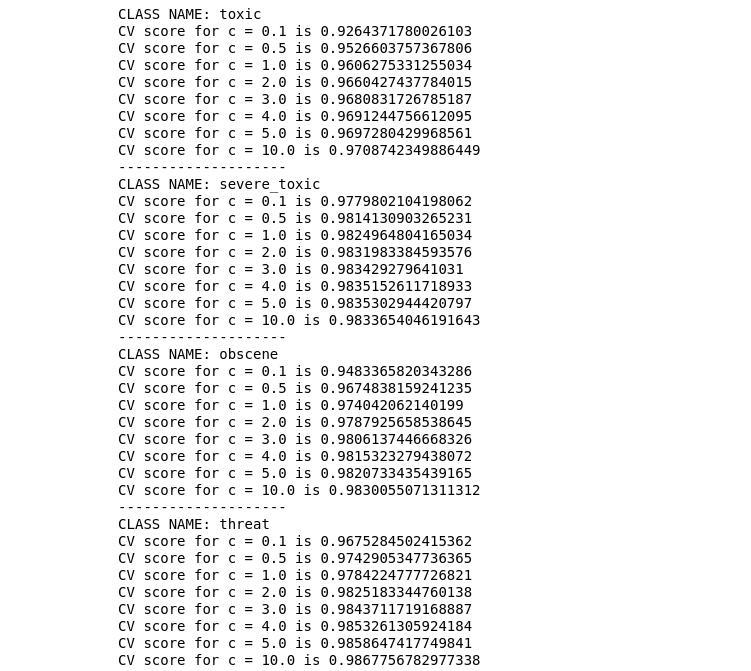
\includegraphics{http://localhost:8888/notebooks/pictures/Toxic_comments1.jpg}
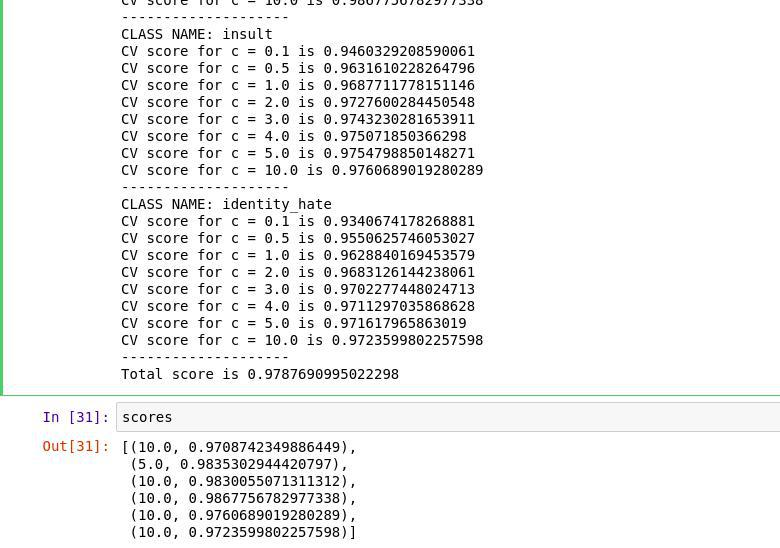
\includegraphics{http://localhost:8888/notebooks/pictures/Toxic_comments2.jpg}
\#\#\# 2
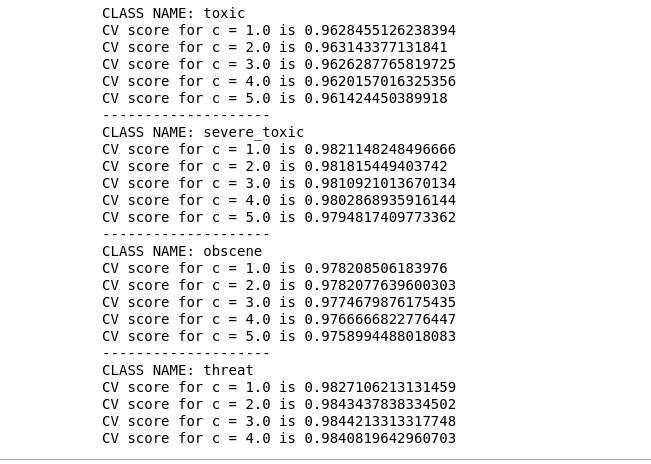
\includegraphics{http://localhost:8888/notebooks/pictures/Toxic_comments3.jpg}

    Попробуйте подобрать лучшие параметры для \texttt{word\_vectorizer} и
\texttt{classifier} оптимизируя метрику
\href{https://en.wikipedia.org/wiki/Receiver_operating_characteristic}{ROC
AUC}

    \begin{center}\rule{0.5\linewidth}{\linethickness}\end{center}

    Опубликуйте лучшие решение на
\href{https://www.kaggle.com/c/jigsaw-toxic-comment-classification-challenge/submit}{Kaggle
Toxic Comment Classification Challenge}

    \begin{Verbatim}[commandchars=\\\{\}]
{\color{incolor}In [{\color{incolor}19}]:} \PY{n}{submission} \PY{o}{=} \PY{n}{pd}\PY{o}{.}\PY{n}{DataFrame}\PY{o}{.}\PY{n}{from\PYZus{}dict}\PY{p}{(}\PY{p}{\PYZob{}}\PY{l+s+s1}{\PYZsq{}}\PY{l+s+s1}{id}\PY{l+s+s1}{\PYZsq{}}\PY{p}{:} \PY{n}{test}\PY{p}{[}\PY{l+s+s1}{\PYZsq{}}\PY{l+s+s1}{id}\PY{l+s+s1}{\PYZsq{}}\PY{p}{]}\PY{p}{\PYZcb{}}\PY{p}{)}
\end{Verbatim}


    \begin{Verbatim}[commandchars=\\\{\}]
{\color{incolor}In [{\color{incolor}20}]:} \PY{n}{c\PYZus{}values} \PY{o}{=} \PY{p}{[}\PY{n}{item}\PY{p}{[}\PY{l+m+mi}{0}\PY{p}{]} \PY{k}{for} \PY{n}{item} \PY{o+ow}{in} \PY{n}{scores}\PY{p}{]}
         
         \PY{k}{for} \PY{n}{class\PYZus{}name}\PY{p}{,} \PY{n}{c} \PY{o+ow}{in} \PY{n+nb}{zip}\PY{p}{(}\PY{n}{class\PYZus{}names}\PY{p}{,} \PY{n}{c\PYZus{}values}\PY{p}{)}\PY{p}{:}
             
             \PY{n}{classifier} \PY{o}{=} \PY{n}{LogisticRegression}\PY{p}{(}\PY{n}{C}\PY{o}{=}\PY{n}{c}\PY{p}{,} \PY{n}{random\PYZus{}state}\PY{o}{=}\PY{l+m+mi}{32}\PY{p}{)}
             
             \PY{n}{y\PYZus{}train} \PY{o}{=} \PY{n}{train}\PY{p}{[}\PY{n}{class\PYZus{}name}\PY{p}{]}
             \PY{n}{classifier}\PY{o}{.}\PY{n}{fit}\PY{p}{(}\PY{n}{x\PYZus{}train}\PY{p}{,} \PY{n}{y\PYZus{}train}\PY{p}{)}
             
             \PY{n}{submission}\PY{p}{[}\PY{n}{class\PYZus{}name}\PY{p}{]} \PY{o}{=} \PY{n}{classifier}\PY{o}{.}\PY{n}{predict\PYZus{}proba}\PY{p}{(}\PY{n}{x\PYZus{}test}\PY{p}{)}\PY{p}{[}\PY{p}{:}\PY{p}{,} \PY{l+m+mi}{1}\PY{p}{]}    
\end{Verbatim}


    \begin{Verbatim}[commandchars=\\\{\}]
{\color{incolor}In [{\color{incolor}21}]:} \PY{n}{submission}\PY{o}{.}\PY{n}{head}\PY{p}{(}\PY{p}{)}
\end{Verbatim}


\begin{Verbatim}[commandchars=\\\{\}]
{\color{outcolor}Out[{\color{outcolor}21}]:}                  id
         0  00001cee341fdb12
         1  0000247867823ef7
         2  00013b17ad220c46
         3  00017563c3f7919a
         4  00017695ad8997eb
\end{Verbatim}
            
    \begin{Verbatim}[commandchars=\\\{\}]
{\color{incolor}In [{\color{incolor}22}]:} \PY{n}{submission}\PY{o}{.}\PY{n}{to\PYZus{}csv}\PY{p}{(}\PY{l+s+s1}{\PYZsq{}}\PY{l+s+s1}{submission.csv}\PY{l+s+s1}{\PYZsq{}}\PY{p}{,} \PY{n}{index}\PY{o}{=}\PY{k+kc}{False}\PY{p}{)}
\end{Verbatim}



    % Add a bibliography block to the postdoc
    
    
    
    \end{document}
